% Created 2017-11-09 Thu 16:38
\documentclass{beamer}
\usepackage{fixltx2e}
\usepackage{graphicx}
\usepackage{longtable}
\usepackage{float}
\usepackage{wrapfig}
\usepackage{soul}
\usepackage{textcomp}
\usepackage{marvosym}
\usepackage{wasysym}
\usepackage{latexsym}
\usepackage{amssymb}
\usepackage{hyperref}
\tolerance=1000
\usepackage{etex}
\usepackage{amsmath}
\usepackage{pstricks}
\usepackage{pgfplots}
\usepackage{tikz}
\usepackage[europeanresistors,americaninductors]{circuitikz}
\usepackage{colortbl}
\usepackage{yfonts}
\usetikzlibrary{shapes,arrows}
\usetikzlibrary{positioning}
\usetikzlibrary{arrows,shapes}
\usetikzlibrary{intersections}
\usetikzlibrary{calc,patterns,decorations.pathmorphing,decorations.markings}
\usepackage[BoldFont,SlantFont,CJKchecksingle]{xeCJK}
\setCJKmainfont[BoldFont=Evermore Hei]{Evermore Kai}
\setCJKmonofont{Evermore Kai}
\usepackage{pst-node}
\usepackage{pst-plot}
\psset{unit=5mm}
\usepackage{beamerarticle}
\mode<beamer>{\usetheme{Frankfurt}}
\mode<beamer>{\usecolortheme{dove}}
\mode<article>{\hypersetup{colorlinks=true,pdfborder={0 0 0}}}
\AtBeginSection[]{\begin{frame}<beamer>\frametitle{Topic}\tableofcontents[currentsection]\end{frame}}
\setbeamercovered{transparent}
\providecommand{\alert}[1]{\textbf{#1}}

\title{机器学习的基本概念}
\author{}
\date{}
\hypersetup{
  pdfkeywords={},
  pdfsubject={},
  pdfcreator={Emacs Org-mode version 7.9.3f}}

\begin{document}

\maketitle

\begin{frame}
\frametitle{Outline}
\setcounter{tocdepth}{3}
\tableofcontents
\end{frame}













\section{课程简介}
\label{sec-1}
\begin{frame}
\frametitle{机器学习}
\label{sec-1-1}
\begin{block}{定义}
\label{sec-1-1-1}

 对于某类任务 $T$ 和性能度量 $P$ 如果一个计算机程序在T上以P衡量的性能随着经验E而自我完善,那么我们称这个计算机程序在从经验E学习。
\end{block}
\end{frame}
\begin{frame}
\frametitle{课程主要内容}
\label{sec-1-2}


\begin{itemize}
\item 概念学习
\item 决策树学习
\item 人工神经网络
\item 评估假设
\item 贝叶斯学习
\item 计算学习理论
\item 基于实例的学习
\item 遗传算法
\item 增强学习
\end{itemize}
\end{frame}
\begin{frame}
\frametitle{与其它课程关系}
\label{sec-1-3}


\begin{itemize}
\item 概率与数理统计
\item 人工智能
\item 模式识别
\item 数据挖掘
\item 最优化理论与方法
\item 控制理论
\item 生物学
\item 心理学
\item 哲学
\end{itemize}
\end{frame}
\section{机器学习示例}
\label{sec-2}
\begin{frame}
\frametitle{机器学习示例}
\label{sec-2-1}

\begin{itemize}
\item 无人驾驶汽车
\item 手写识别
\item 人脸识别
\item 垃圾邮件过滤
\end{itemize}
\end{frame}
\begin{frame}
\frametitle{Typical Datamining Task}
\label{sec-2-2}


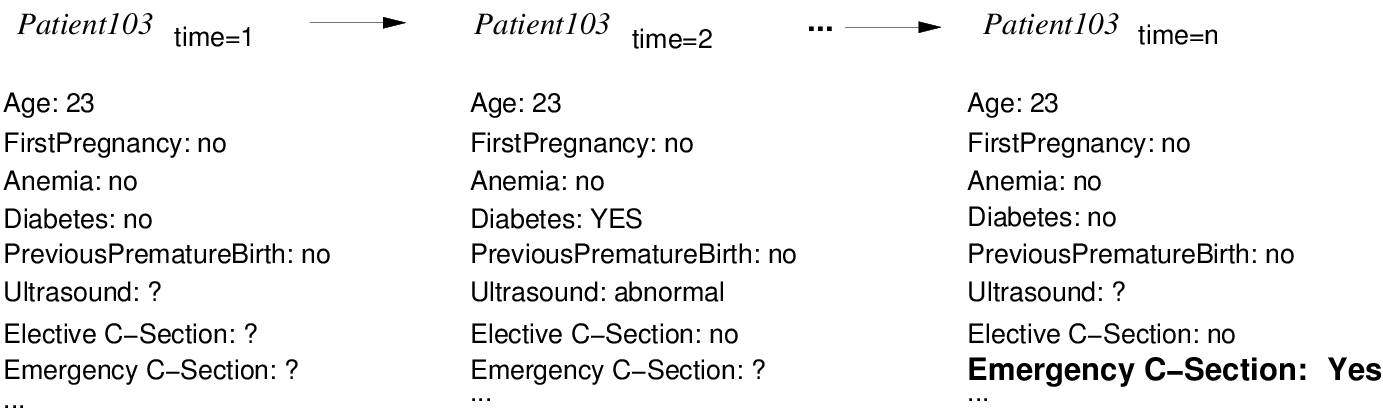
\includegraphics[width=.9\linewidth]{./image/csec.png}

\begin{itemize}
\item Given:
\begin{itemize}
\item 9714 patient records, each describing a pregnancy and birth
\item Each patient record contains 215 features
\end{itemize}
\item Learn to predict:
\begin{itemize}
\item item Classes of future patients at high risk for Emergency Cesarean Section
\end{itemize}
\end{itemize}
\end{frame}
\begin{frame}[fragile]
\frametitle{Datamining Result}
\label{sec-2-3}


\begin{itemize}
\item Data:
\end{itemize}

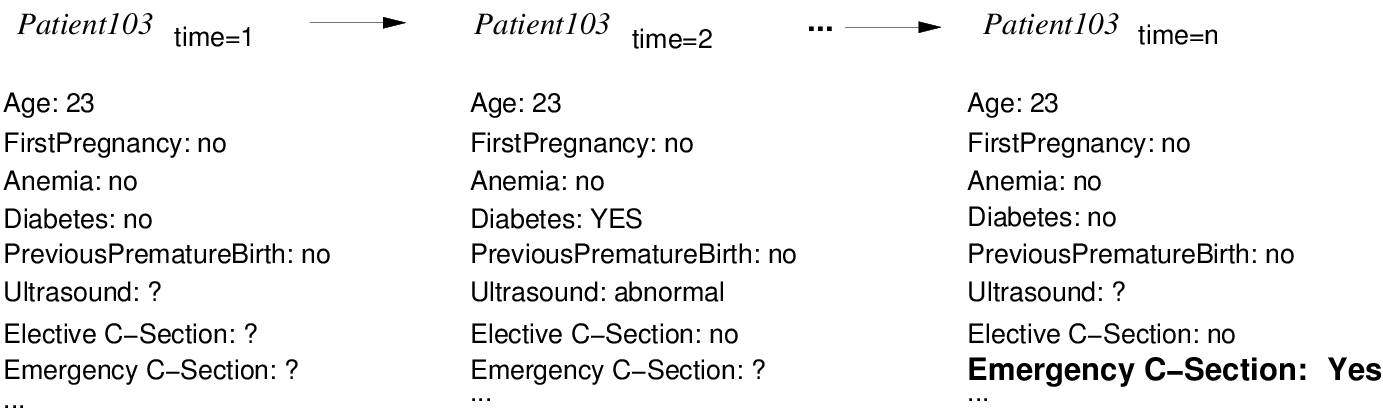
\includegraphics[width=.9\linewidth]{./image/csec.png}

\begin{itemize}
\item One of 18 learned rules:
       \begin{verbatim}
       If   No previous vaginal delivery, and
            Abnormal 2nd Trimester Ultrasound, and
            Malpresentation at admission
       Then Probability of Emergency C-Section is 0.6
       
        Over training data: 26/41 = .63, 
        Over test data: 12/20 = .60
       \end{verbatim}
\end{itemize}
\end{frame}
\begin{frame}[fragile]
\frametitle{Credit Risk Analysis}
\label{sec-2-4}

Data:

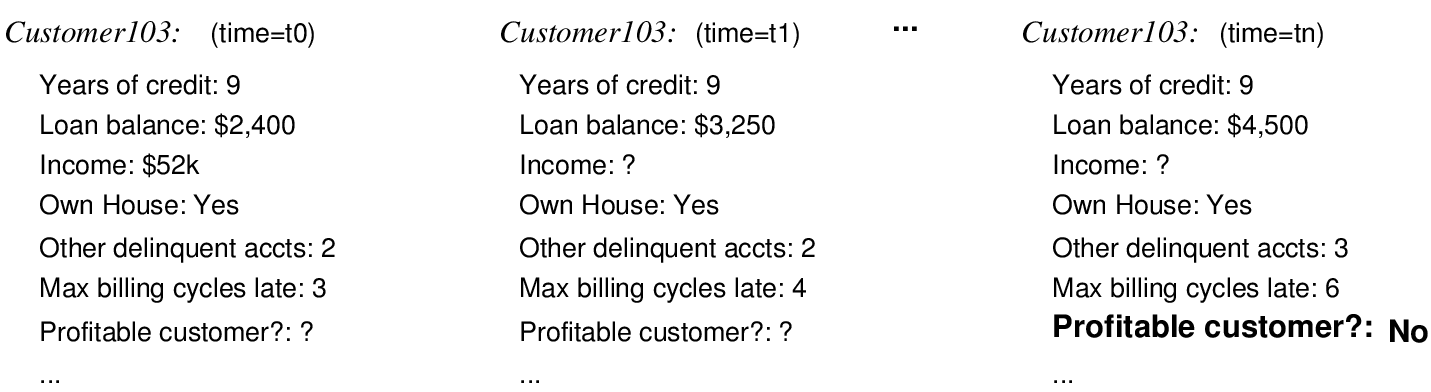
\includegraphics[width=.9\linewidth]{./image/credit-outcomes.png}

Rules learned from synthesized data:
\begin{verbatim}
If   Other-Delinquent-Accounts > 2, and
     Number-Delinquent-Billing-Cycles > 1
Then Profitable-Customer? = No
     [Deny Credit Card application]

If   Other-Delinquent-Accounts = 0, and
     (Income > $30k)  OR  (Years-of-Credit > 3)
Then Profitable-Customer? = Yes
     [Accept Credit Card application]
\end{verbatim}
\end{frame}
\begin{frame}
\frametitle{Customer purchase behavior:}
\label{sec-2-5}

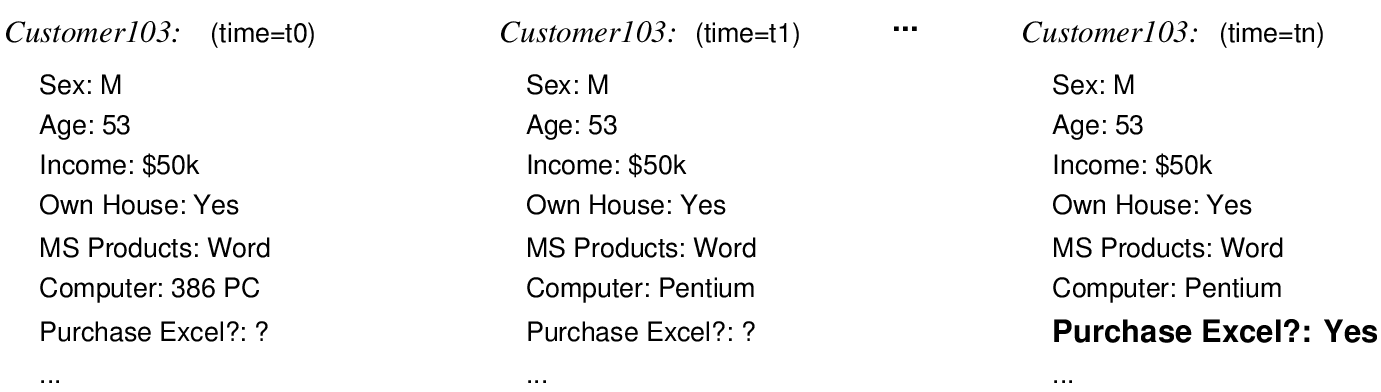
\includegraphics[width=.9\linewidth]{./image/customer-outcomes.png}
\end{frame}
\begin{frame}
\frametitle{Customer retention:}
\label{sec-2-6}


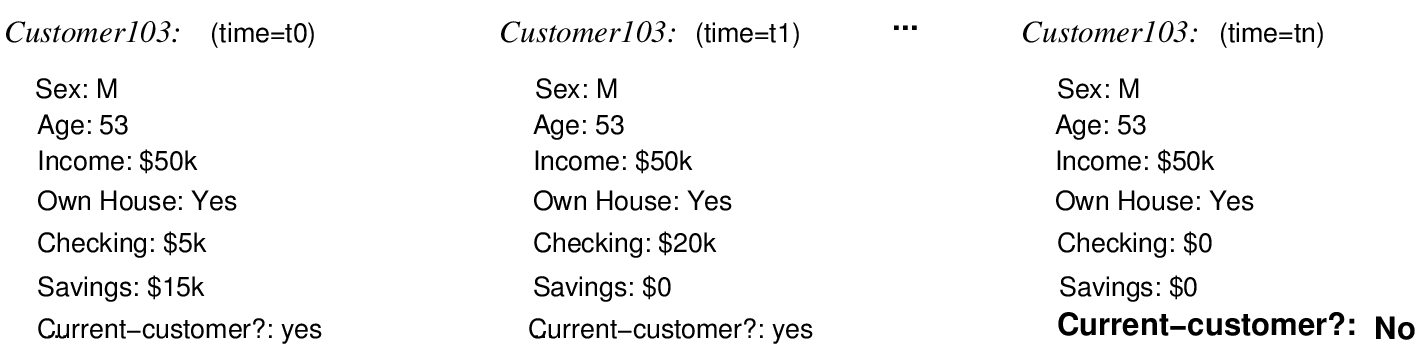
\includegraphics[width=.9\linewidth]{./image/bank-customer.png}
\end{frame}
\begin{frame}
\frametitle{Process optimization:}
\label{sec-2-7}

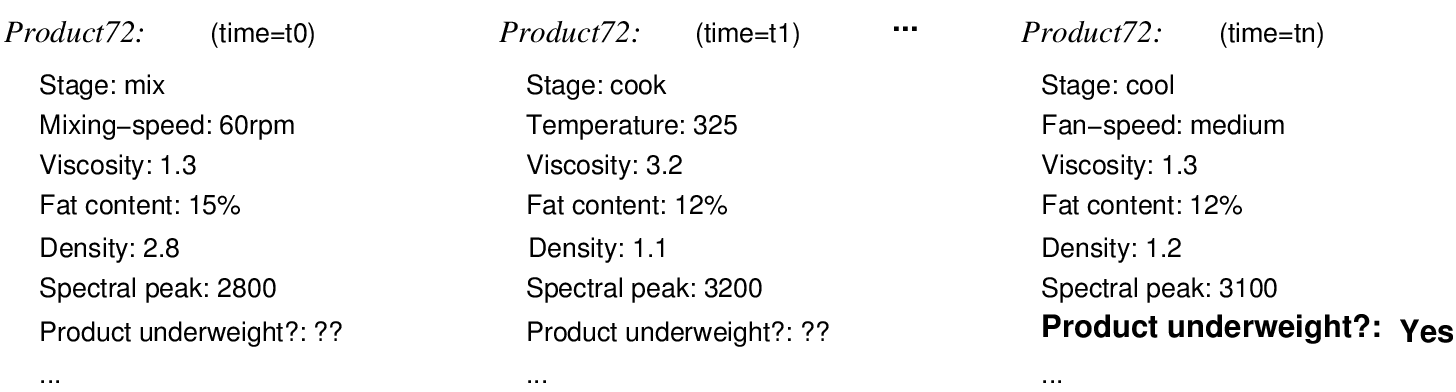
\includegraphics[width=.9\linewidth]{./image/process-outcomes.png}
\end{frame}
\begin{frame}
\frametitle{ALVINN [Pomerleau] drives 70 mph on highways}
\label{sec-2-8}


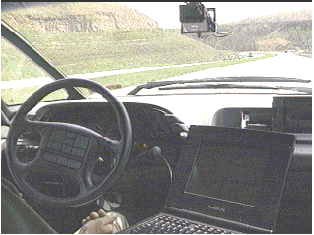
\includegraphics[width=0.3\textwidth]{./image/nl5-interior-front-color.png}
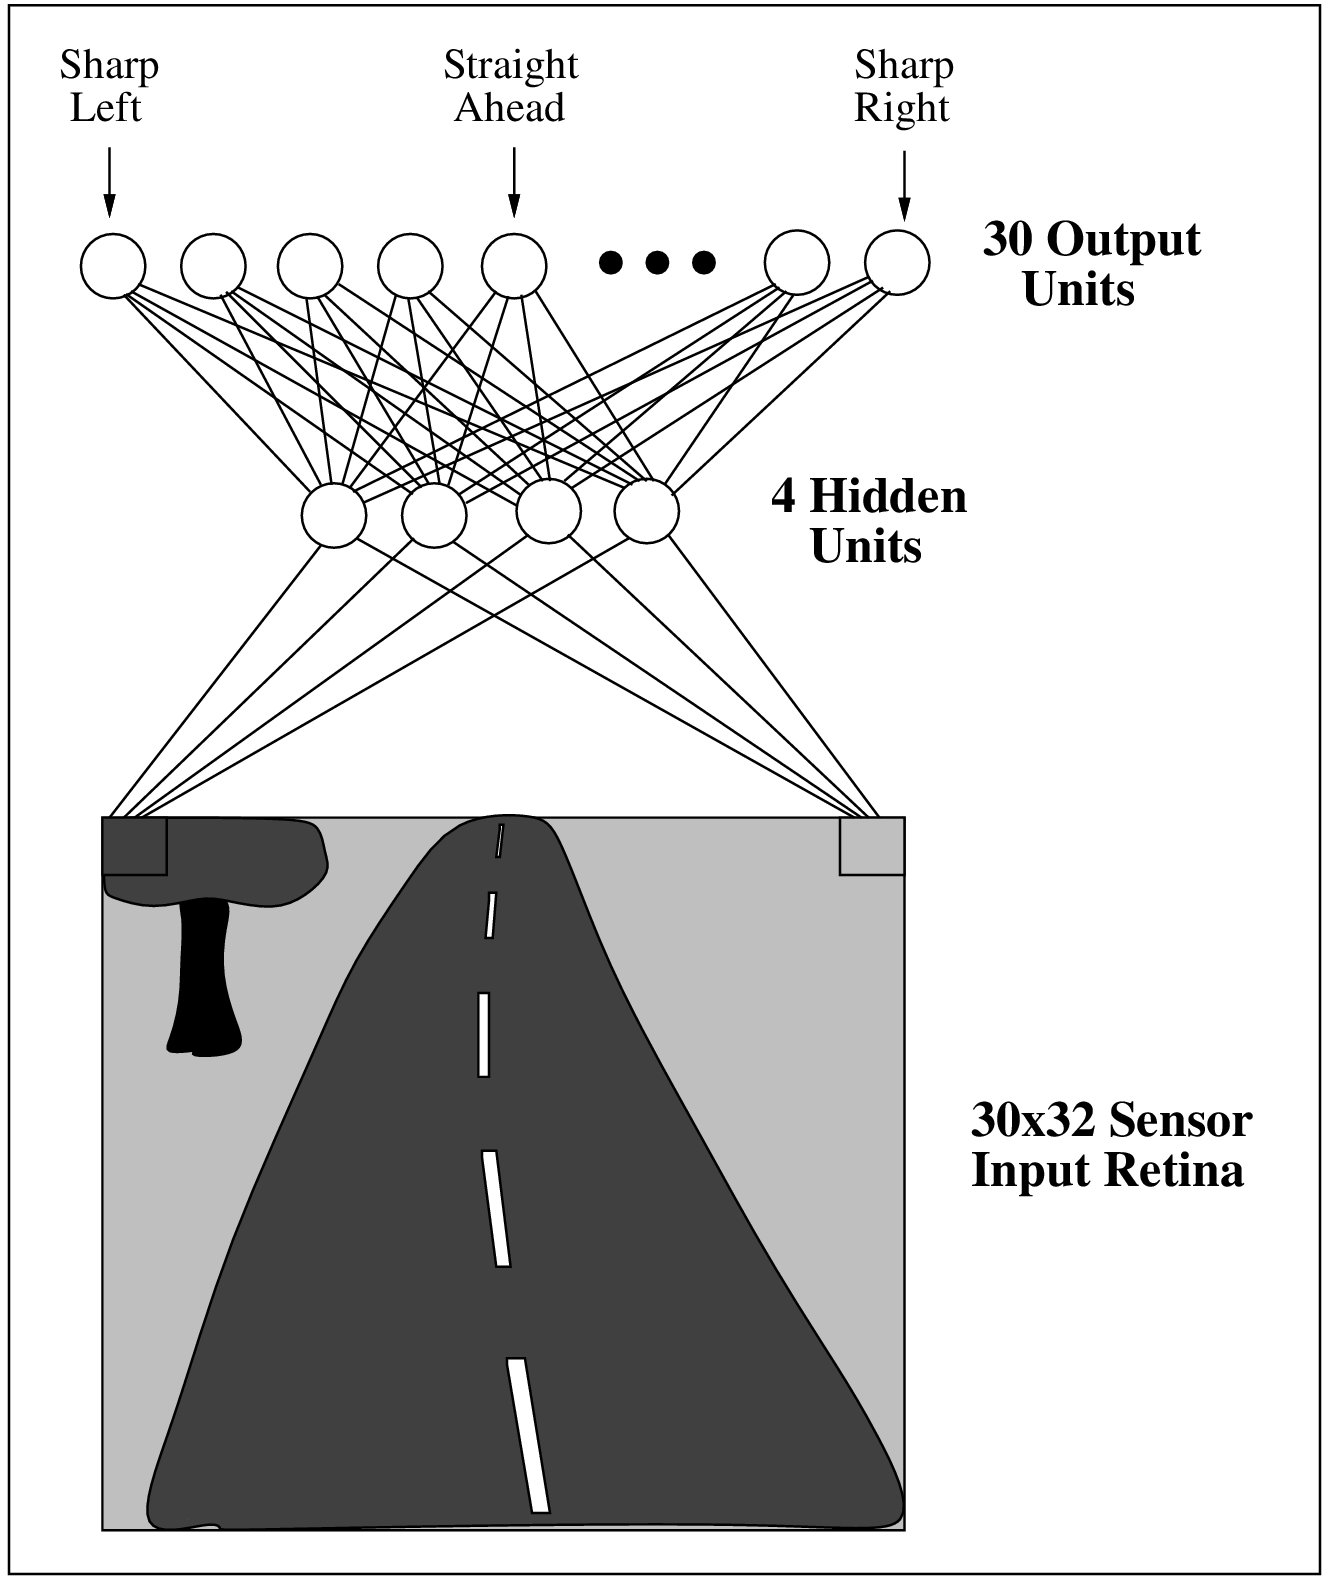
\includegraphics[width=0.3\textwidth]{./image/alvinn1.png}
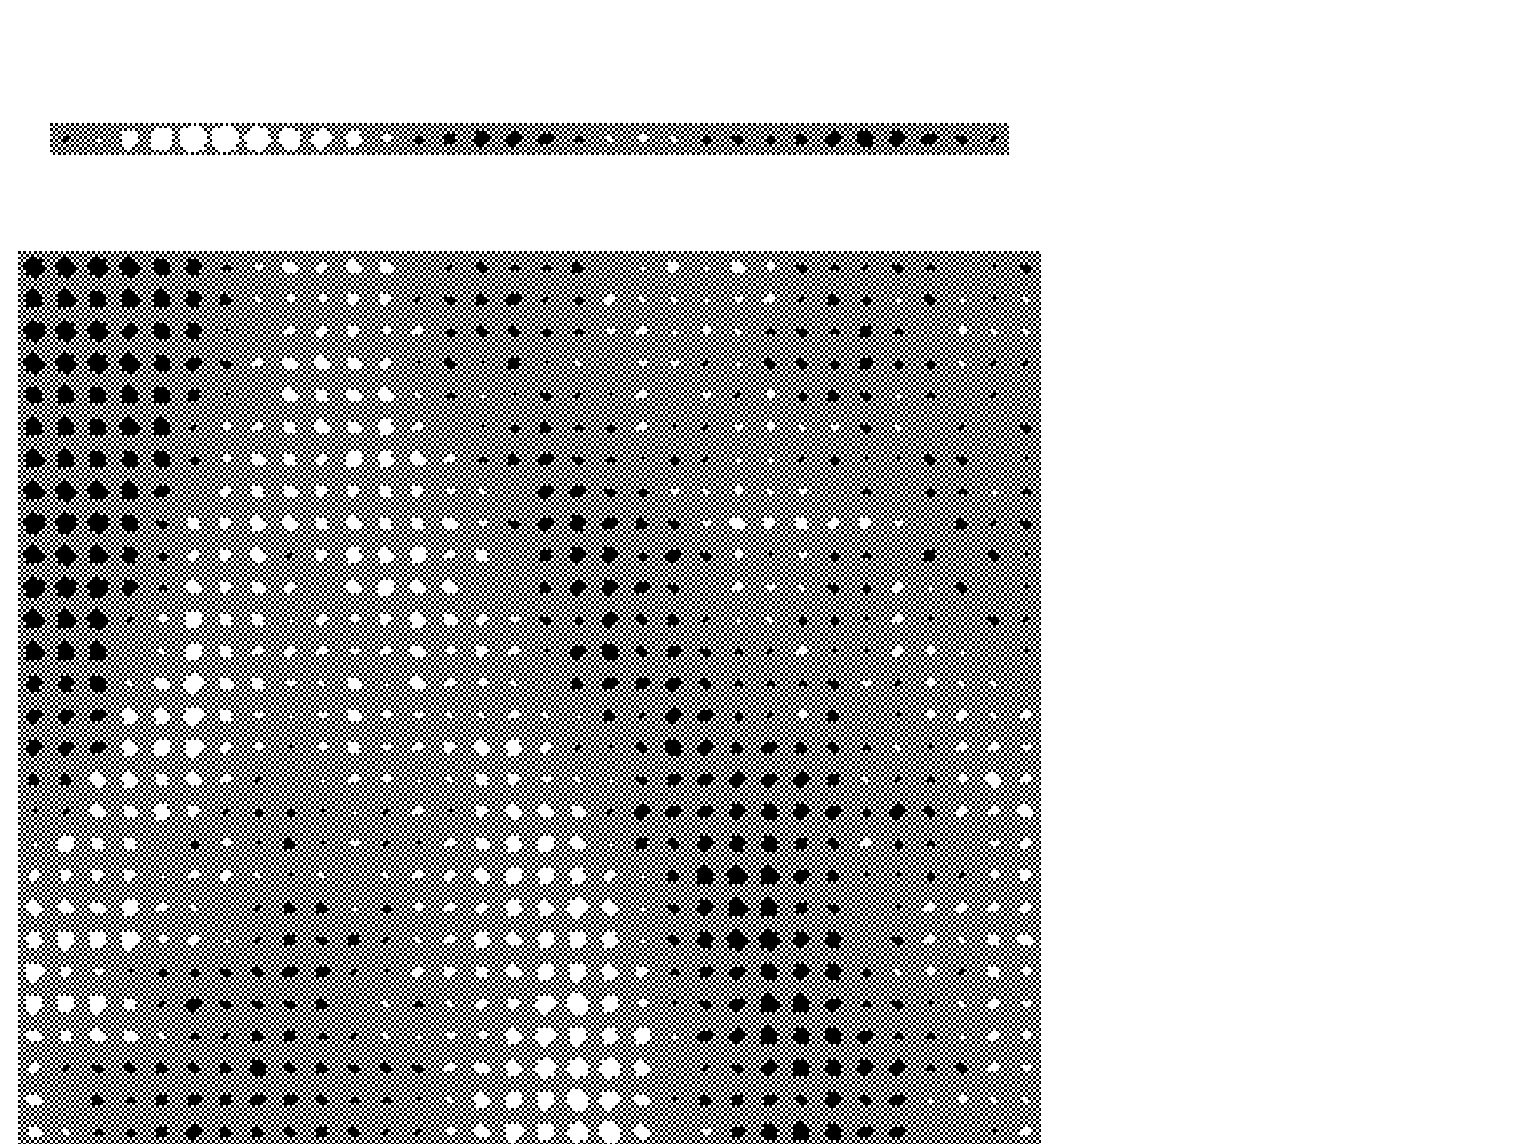
\includegraphics[width=0.3\textwidth]{./image/alvinn2.png}
\end{frame}
\begin{frame}
\frametitle{Software that Customizes to User}
\label{sec-2-9}

\center
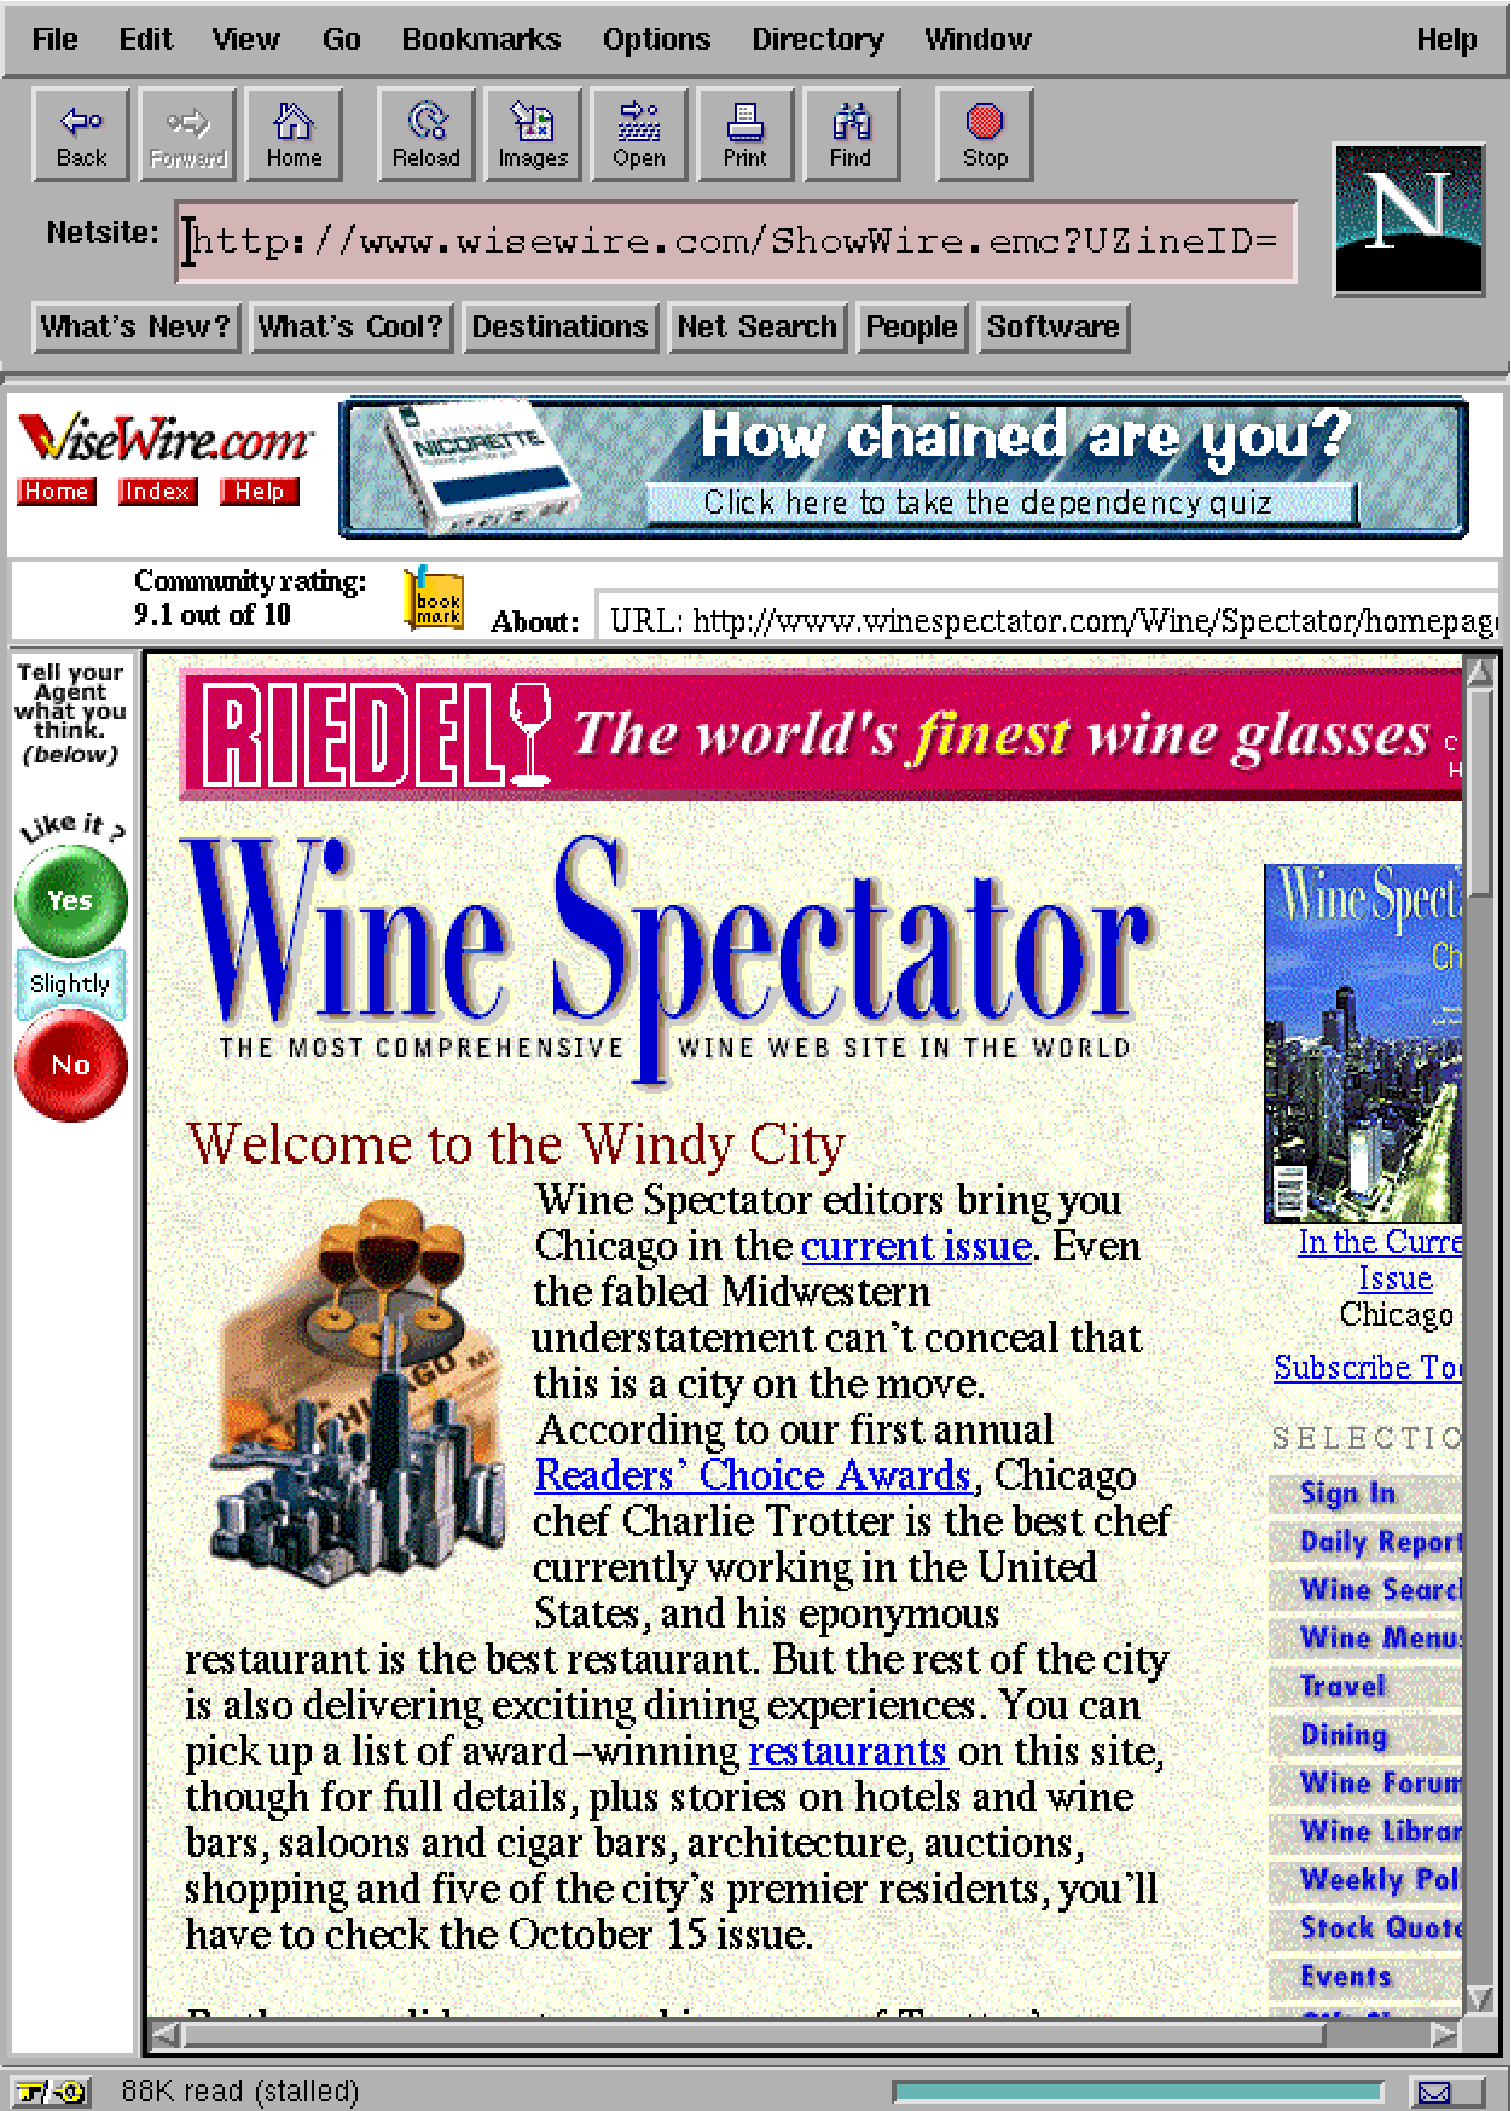
\includegraphics[width=0.5\textwidth]{./image/wisewire.png}

\centerline{[[http://www.wisewire.com][http://www.wisewire.com]]}
\end{frame}
\section{学习问题的标准描述}
\label{sec-3}
\begin{frame}
\frametitle{定义}
\label{sec-3-1}

对于某类任务 $T$ 和性能度量 $P$ ,如果一个计算机程序在 $T$ 上以 $P$ 衡量的性能随着经验 $E$ 而自我完善,那么我们称这个计算机程序在从经验 $E$ 学习。

\begin{itemize}
\item 例如, 对于学习下西洋跳棋的计算机程序,它可以通过和自己下棋获取经验,它担负的任务是参与西洋跳棋对弈,它的性能用它赢棋的能力来衡量。
\item 通常,为了很好地定义一个学习问题,我们必须明确这样三个特征:
\begin{itemize}
\item 任务的种类;
\item 衡量任务提高的标准;
\item 经验的来源。
\end{itemize}
\end{itemize}
\end{frame}
\begin{frame}
\frametitle{西洋跳棋学习问题:}
\label{sec-3-2}

\begin{itemize}
\item 任务T:下西洋跳棋
\item 性能标准P:比赛中击败对手的百分比
\item 训练经验E:和自己进行对弈
\end{itemize}
\end{frame}
\begin{frame}
\frametitle{手写识别学习问题}
\label{sec-3-3}

\begin{itemize}
\item 任务T:识别和分类图像中的手写文字
\item 性能标准P:分类的正确率
\item 训练经验E:已知分类的手写文字数据库
\end{itemize}
\end{frame}
\begin{frame}
\frametitle{机器人驾驶学习问题}
\label{sec-3-4}

\begin{itemize}
\item 任务T:通过视觉传感器在四车道高速公路上驾驶
\item 性能标准P:平均无差错行驶里程(差错由人类的监督裁定)
\item 训练经验E:注视人类驾驶时录制的一系列图像和驾驶指令
\end{itemize}
\end{frame}
\section{设计一个学习系统}
\label{sec-4}
\begin{frame}
\frametitle{西洋跳棋学习问题:}
\label{sec-4-1}

\begin{itemize}
\item 任务T:下西洋跳棋
\item 性能标准P:世界锦标赛上击败对手的百分比
\item 训练经验E:和自己进行对弈
\end{itemize}

为了完成这个学习系统的设计,现在需要选择:
\begin{itemize}
\item 要学习的经验
\item 要学习的知识的确切类型
\item 对于这个目标知识的表示
\item 一种学习机制
\end{itemize}
\end{frame}
\begin{frame}
\frametitle{选取训练经验的类型}
\label{sec-4-2}

\begin{itemize}
\item 直接或间接
\begin{itemize}
\item 直接的(direct)训练样例,即各种棋盘状态和相应的正确走子中学习。
\item 间接(indirect)的信息,包含很多过去的对弈序列和最终结局。(关于较早走子的正确性必须从对弈最终的输赢来推断。)
\end{itemize}
\item 有无施教者
\begin{itemize}
\item 学习器可能依赖施教者选取棋盘状态,和提供每一次的正确移动。或者,学习器可能自己提出它认为特别困惑的棋局并向施教者询问正确的走子。
\item 或者,学习器可以完全控制棋局和(间接的)训练分类,就像没有施教者时它和自己对弈进行学习一样。
\end{itemize}
\item 训练样例的分布是否代表实例分布
\end{itemize}
\end{frame}
\begin{frame}
\frametitle{选择目标函数}
\label{sec-4-3}

\begin{itemize}
\item 目标函数1, 对任何给定的棋局(合法棋局集合中的棋盘状态)能选出最好的走法(从合法走子集合中产生某个走子作为输出)
   $$ChooseMove: Board \rightarrow Move$$
\item 目标函数2(评估函数),它为任何给定棋局赋予一个数字的评分
  $$V: Board \rightarrow \Re$$
\end{itemize}
\end{frame}
\begin{frame}
\frametitle{定义目标函数( $V$ )}
\label{sec-4-4}

\begin{itemize}
\item 例:
\begin{itemize}
\item 如果b是一最终的胜局,那么V(b)=100
\item 如果b是一最终的负局,那么V(b)=-100
\item 如果b是一最终的和局,那么V(b)=0
\item 如果b不是最终棋局,那么V(b)=V(b'),其中b'是从b开始双方都采取最优对弈后可达到的终局。
\end{itemize}
\item 注:正确,但不可操作
\end{itemize}
\end{frame}
\begin{frame}
\frametitle{选择目标函数表示}
\label{sec-4-5}


\begin{itemize}
\item 一组规则
\item 神经网络
\item 棋盘状态的多项式函数
\item \ldots{}
\end{itemize}
\end{frame}
\begin{frame}
\frametitle{目标函数表示}
\label{sec-4-6}

\[ w_{0} + w_{1}\cdot bp(b) + w_{2}\cdot rp(b) + w_{3}\cdot bk(b) + w_{4}\cdot rk(b) + w_{5}\cdot bt(b) + w_{6}\cdot rt(b) \]

\begin{itemize}
\item $bp(b)$: number of black pieces on board $b$
\item $rp(b)$: number of red pieces on $b$
\item $bk(b)$: number of black kings on $b$
\item $rk(b)$: number of red kings on $b$
\item $bt(b)$: number of red pieces threatened by black (i.e., which can be taken
         on black's next turn)
\item $rt(b)$:  number of black pieces threatened by red
\end{itemize}
\end{frame}
\begin{frame}
\frametitle{估计训练值}
\label{sec-4-7}


\begin{itemize}
\item $V(b)$: 真实目标函数
\item $\hat{V}(b)$ : 学习到的函数
\item $V_{train}(b)$: 训练值
\item 学习器可以得到的训练信息仅是对弈最后的胜负。
\item 训练值估计法则 
   $$V_{train}(b) \leftarrow \hat{V}(Successor(b))$$
   $Successor(b)$ 表示 一个回合后的棋盘状态。
\end{itemize}
\end{frame}
\begin{frame}
\frametitle{权值调整}
\label{sec-4-8}

LMS 权值更新法则(LMS Weight update rule)
\begin{itemize}
\item Do repeatedly:
\begin{itemize}
\item 随机选取一个训练样例 $b$
\item 使用当前的权值计算 $error(b)$:
         \[error(b) = V_{train}(b) - \hat{V}(b)\]
\item 对每一个权值wi进行如下更新
          \[w_{i} \leftarrow w_{i} + c \cdot f_{i} \cdot error(b) \]
      $c$ 是一个小常数, 如 0.1, 用来调整权值更新的幅度
\end{itemize}
\end{itemize}
\end{frame}
\begin{frame}
\frametitle{最终设计}
\label{sec-4-9}

\center
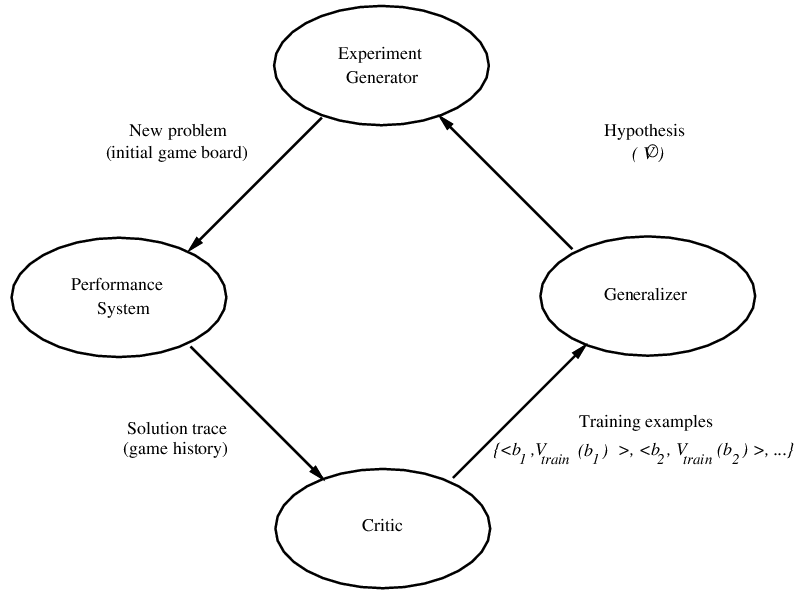
\includegraphics[width=0.7\textwidth]{./image/intro-final-design.png}
\end{frame}
\begin{frame}
\frametitle{最终设计}
\label{sec-4-10}

\begin{itemize}
\item 执行系统(Performance system),这个模块是用学会的目标函数来解决给定的任务,在此就是对弈西洋跳棋。
\end{itemize}
\mode<article>{它把新问题(新一盘棋)的实例作为输入,产生一组解答路线(对弈历史记录)作为输出。
在这里,执行系统采用的选择下一步走法的策略是由学到的评估函数来决定的。
所以我们期待它的性能会随着评估函数的日益准确而提高。}

\begin{itemize}
\item 鉴定器(Critic),它以对弈的路线或历史记录作为输入,输出目标函数的一系列训练样例。
\end{itemize}
如图所示,每一个训练样例对应路线中的某个棋盘状态和目标函数给这个样例的评估值 $V_{train}$ 。

\begin{itemize}
\item 泛化器(Generalizer),它以训练样例作为输入,输出一个假设,作为它对目标函数的估计。
\end{itemize}
它从特定的训练样例中泛化,猜测一个一般函数,使其能够覆盖这些样例以及样例之外的情形。

\begin{itemize}
\item 实验生成器(Experiment Generator),它以当前的假设(当前学到的函数)作为输入,输出一个新的问题(例如,最初的棋局)供执行系统去探索。
\end{itemize}
它的角色是挑选新的练习问题,以使整个系统的学习速率最大化。
\end{frame}
\begin{frame}
\frametitle{设计过程}
\label{sec-4-11}

\center
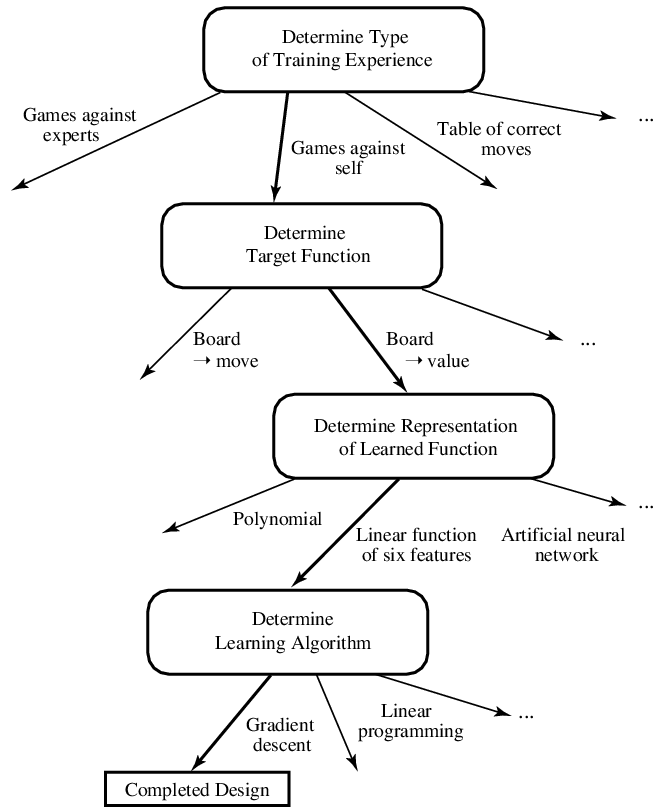
\includegraphics[width=0.5\textwidth]{./image/intro-f1.png}
\end{frame}
\section{机器学习的问题}
\label{sec-5}


\begin{itemize}
\item 从特定的训练数据学习一般的目标函数存在什么样的算法?
\begin{itemize}
\item 如果提供了充足的训练数据,什么样的条件下会使特定的算法收敛到期望的函数?
\item 哪个算法对哪些问题和表示的性能最好。
\end{itemize}
\item 多少训练数据是充足的?
\begin{itemize}
\item 怎样找到学习到的假设的置信度与训练数据的数量及提供给学习器的假设空间特性之间的一般关系?
\end{itemize}
\item 学习器拥有的先验知识是怎样引导从样例进行泛化的过程的?
\begin{itemize}
\item 当先验知识仅仅是近似正确时,它们会有帮助吗?
\end{itemize}
\item 对于选择有用的后续训练经验,什么样的策略最好?
\begin{itemize}
\item 这个策略的选择会怎样影响学习问题的复杂性?
\end{itemize}
\item 怎样把学习任务简化为一个或多个函数逼近问题?
\begin{itemize}
\item 换一种方式,系统该试图学习哪些函数?
\item 这个过程本身能自动化吗?
\end{itemize}
\item 学习器怎样自动地改变表示法来提高表示和学习目标函数的能力?
\end{itemize}
\section{机器学习相关资源}
\label{sec-6}
\begin{frame}
\frametitle{课程}
\label{sec-6-1}


\begin{itemize}
\item \href{https://www.coursera.org/learn/machine-learning}{https://www.coursera.org/learn/machine-learning}  Machine Learning Stanford University (coursera)
\item \href{http://open.163.com/special/opencourse/machinelearning.html}{http://open.163.com/special/opencourse/machinelearning.html}  斯坦福大学公开课 :机器学习课程(网易公开课)
\item \href{http://open.163.com/special/opencourse/learningfromdata.html}{http://open.163.com/special/opencourse/learningfromdata.html} 加州理工学院公开课:机器学习与数据挖掘
\end{itemize}
\end{frame}
\begin{frame}
\frametitle{资料}
\label{sec-6-2}

\begin{itemize}
\item \href{https://www.kaggle.com/}{https://www.kaggle.com/}
    数据科学竞赛平台、社区
\item \href{http://philschatz.com/biology-book/}{http://philschatz.com/biology-book/}  
    a  freedom book about biology
\item \href{http://www.cs.cmu.edu/~tom/mlbook-chapter-slides.html}{http://www.cs.cmu.edu/\textasciitilde tom/mlbook-chapter-slides.html}
    Machine Learning slide (\LaTeX{} source )
\item \href{http://www.cs.cmu.edu/afs/cs.cmu.edu/project/theo-20/www/mlbook/latex-support.html}{http://www.cs.cmu.edu/afs/cs.cmu.edu/project/theo-20/www/mlbook/latex-support.html} 
    Machine Learning slide (\LaTeX{} source )
\item \href{https://learnxinyminutes.com}{https://learnxinyminutes.com}  \textbackslash{}
    各种程序设计语言快速入门
\item \href{http://cos.name/}{http://cos.name/}
    统计技术社区
\item \href{https://databricks.com/}{https://databricks.com/}
    Spark在线学习
\end{itemize}
\end{frame}
\section{工具}
\label{sec-7}
\begin{frame}
\frametitle{C/C++}
\label{sec-7-1}

\begin{itemize}
\item \href{http://dlib.net}{http://dlib.net}
\item \href{http://mlpack.org/}{http://mlpack.org/}
\item \href{http://opencv.org/}{http://opencv.org/}
\item \href{http://caffe.berkeleyvision.org}{http://caffe.berkeleyvision.org}
\item \href{http://mxnet.io/}{http://mxnet.io/}
\end{itemize}
\end{frame}
\begin{frame}
\frametitle{Lua}
\label{sec-7-2}

\begin{itemize}
\item \href{http://torch.ch}{http://torch.ch}
\item \href{https://github.com/torchnet/}{https://github.com/torchnet/}
\end{itemize}
\end{frame}
\begin{frame}
\frametitle{Python}
\label{sec-7-3}

\begin{itemize}
\item \href{http://scikit-learn.org/}{http://scikit-learn.org/}
\item \href{https://www.tensorflow.org}{https://www.tensorflow.org}
\item \href{http://www.deeplearning.net/software/theano/}{http://www.deeplearning.net/software/theano/}
\item \href{https://github.com/NervanaSystems/neon}{https://github.com/NervanaSystems/neon}
\end{itemize}
\end{frame}
\begin{frame}
\frametitle{Java}
\label{sec-7-4}

\begin{itemize}
\item \href{http://www.cs.waikato.ac.nz/ml/weka/index.html}{http://www.cs.waikato.ac.nz/ml/weka/index.html}
\item \href{http://moa.cms.waikato.ac.nz/}{http://moa.cms.waikato.ac.nz/}
\item \href{http://spark.apache.org/mllib/}{http://spark.apache.org/mllib/}
\item \href{https://mahout.apache.org/}{https://mahout.apache.org/}
\item \href{http://www.h2o.ai/}{http://www.h2o.ai/}
\item \href{http://deeplearning4j.org/}{http://deeplearning4j.org/}
\item \href{http://neuroph.sourceforge.net/}{http://neuroph.sourceforge.net/}
\item \href{http://airbnb.io/aerosolve/}{http://airbnb.io/aerosolve/}
\end{itemize}
\end{frame}
\begin{frame}
\frametitle{科学计算}
\label{sec-7-5}

\begin{itemize}
\item Rstudio(R)
\item Matlab/Octave
\item Scilab
\item Sage
\item Julia
\item Spyder(Python)
\item RapidMiner \href{https://rapidminer.com/}{https://rapidminer.com/}
\end{itemize}
\end{frame}

\end{document}
